%package list
\documentclass{article}
\usepackage[top=3cm, bottom=3cm, outer=3cm, inner=3cm]{geometry}
\usepackage{multicol}
\usepackage{graphicx}
\usepackage{url}
%\usepackage{cite}
\usepackage{hyperref}
\usepackage{array}
%\usepackage{multicol}
\newcolumntype{x}[1]{>{\centering\arraybackslash\hspace{0pt}}p{#1}}
\usepackage{natbib}
\usepackage{pdfpages}
\usepackage{multirow}
\usepackage[normalem]{ulem}
\useunder{\uline}{\ul}{}
\usepackage{svg}
\usepackage{xcolor}
\usepackage{listings}
\lstdefinestyle{ascii-tree}{
	literate={├}{|}1 {─}{--}1 {└}{+}1 
}
\lstset{basicstyle=\ttfamily,
	showstringspaces=false,
	commentstyle=\color{red},
	keywordstyle=\color{blue}
}
%\usepackage{booktabs}
\usepackage{caption}
\usepackage{subcaption}
\usepackage{float}
\usepackage{array}

\newcolumntype{M}[1]{>{\centering\arraybackslash}m{#1}}
\newcolumntype{N}{@{}m{0pt}@{}}


%%%%%%%%%%%%%%%%%%%%%%%%%%%%%%%%%%%%%%%%%%%%%%%%%%%%%%%%%%%%%%%%%%%%%%%%%%%%
%%%%%%%%%%%%%%%%%%%%%%%%%%%%%%%%%%%%%%%%%%%%%%%%%%%%%%%%%%%%%%%%%%%%%%%%%%%%
\newcommand{\itemEmail}{jchuraaca@unsa.edu.pe}
\newcommand{\itemStudent}{Julio Rubén Chura Acabana}
\newcommand{\itemCourse}{ F. de Programción 2}
\newcommand{\itemCourseCode}{20230472}
\newcommand{\itemSemester}{I}
\newcommand{\itemUniversity}{Universidad Nacional de San Agustín de Arequipa}
\newcommand{\itemFaculty}{Facultad de Ingeniería de Producción y Servicios}
\newcommand{\itemDepartment}{Departamento Académico de Ingeniería de Sistemas e Informática}
\newcommand{\itemSchool}{Escuela Profesional de Ingeniería de Sistemas}
\newcommand{\itemAcademic}{2023 - B}
\newcommand{\itemInput}{Del 10 de Enero 2023}
\newcommand{\itemOutput}{Al 15 de Enero 2023}
\newcommand{\itemPracticeNumber}{22}
\newcommand{\itemTheme}{Interfaz Gráfica de Usuario}
%%%%%%%%%%%%%%%%%%%%%%%%%%%%%%%%%%%%%%%%%%%%%%%%%%%%%%%%%%%%%%%%%%%%%%%%%%%%
%%%%%%%%%%%%%%%%%%%%%%%%%%%%%%%%%%%%%%%%%%%%%%%%%%%%%%%%%%%%%%%%%%%%%%%%%%%%

\usepackage[english,spanish]{babel}
\usepackage[utf8]{inputenc}
\AtBeginDocument{\selectlanguage{spanish}}
\renewcommand{\figurename}{Figura}
\renewcommand{\refname}{Referencias}
\renewcommand{\tablename}{Tabla} %esto no funciona cuando se usa babel
\AtBeginDocument{%
	\renewcommand\tablename{Tabla}
}

\usepackage{fancyhdr}
\pagestyle{fancy}
\fancyhf{}
\setlength{\headheight}{30pt}
\renewcommand{\headrulewidth}{1pt}
\renewcommand{\footrulewidth}{1pt}
\fancyhead[L]{\raisebox{-0.2\height}{
\includegraphics[width=3cm]{img/logo_episunsa.png}}}
\fancyhead[C]{\fontsize{7}{7}\selectfont	\itemUniversity \\ \itemFaculty \\ \itemDepartment \\ \itemSchool \\ \textbf{\itemCourse}}
\fancyhead[R]{\raisebox{-0.2\height}{
\includegraphics[width=1.2cm]{img/logo_abet}}}
\fancyfoot[L]{Estudiante Julio Rubén Chura Acabana}
\fancyfoot[C]{\itemCourse}
\fancyfoot[R]{Página \thepage}

% para el codigo fuente
\usepackage{listings}
\usepackage{color, colortbl}
\definecolor{dkgreen}{rgb}{0,0.6,0}
\definecolor{gray}{rgb}{0.5,0.5,0.5}
\definecolor{mauve}{rgb}{0.58,0,0.82}
\definecolor{codebackground}{rgb}{0.95, 0.95, 0.92}
\definecolor{tablebackground}{rgb}{0.8, 0, 0}

\lstset{frame=tb,
	language=bash,
	aboveskip=3mm,
	belowskip=3mm,
	showstringspaces=false,
	columns=flexible,
	basicstyle={\small\ttfamily},
	numbers=none,
	numberstyle=\tiny\color{gray},
	keywordstyle=\color{blue},
	commentstyle=\color{dkgreen},
	stringstyle=\color{mauve},
	breaklines=true,
	breakatwhitespace=true,
	tabsize=3,
	backgroundcolor= \color{codebackground},
}

\begin{document}
	
	\vspace*{10px}
	
	\begin{center}	
		\fontsize{17}{17} \textbf{ Informe de Laboratorio \itemPracticeNumber}
	\end{center}
	\centerline{\textbf{\Large Tema: \itemTheme}}
	%\vspace*{0.5cm}	
	
	\begin{flushright}
		\begin{tabular}{|M{2.5cm}|N|}
			\hline 
			\rowcolor{tablebackground}
			\color{white} \textbf{Nota}  \\
			\hline 
			\\[30pt]
			\hline 			
		\end{tabular}
	\end{flushright}	
	
	\begin{table}[H]
		\begin{tabular}{|x{4.7cm}|x{4.8cm}|x{4.8cm}|}
			\hline 
			\rowcolor{tablebackground}
			\color{white} \textbf{Estudiante} & \color{white}\textbf{Escuela}  & \color{white}\textbf{Asignatura}   \\
			\hline 
			{\itemStudent \par \itemEmail} & \itemSchool & {\itemCourse \par Semestre: \itemSemester \par Código: \itemCourseCode}     \\
			\hline 			
		\end{tabular}
	\end{table}		
	
	\begin{table}[H]
		\begin{tabular}{|x{4.7cm}|x{4.8cm}|x{4.8cm}|}
			\hline 
			\rowcolor{tablebackground}
			\color{white}\textbf{Laboratorio} & \color{white}\textbf{Tema}  & \color{white}\textbf{Duración}   \\
			\hline 
			\itemPracticeNumber & \itemTheme & 04 horas   \\
			\hline 
		\end{tabular}
	\end{table}
	
	\begin{table}[H]
		\begin{tabular}{|x{4.7cm}|x{4.8cm}|x{4.8cm}|}
			\hline 
			\rowcolor{tablebackground}
			\color{white}\textbf{Semestre académico} & \color{white}\textbf{Fecha de inicio}  & \color{white}\textbf{Fecha de entrega}   \\
			\hline 
			\itemAcademic & \itemInput &  \itemOutput  \\
			\hline 
		\end{tabular}
	\end{table}
	
	\section{Tarea}
	\begin{itemize}		
		\item Cree una versión del videojuego de estrategia usando componentes básicos GUI: Etiquetas, botones,
		cuadros de texto, JOptionPane, Color.
	\end{itemize}
	
	\section{Equipos, materiales y temas utilizados}
	\begin{itemize}
		\item Sistema Operativo Windows
		\item Visual Studio Code 1.85.1
		\item OpenJDK 64-Bits 20.0.2.
		\item Git 2.42.0.
		\item Cuenta en GitHub con el correo institucional.
		\item Herencia y Polimorfismo
	\end{itemize}
	
	\section{URL de Repositorio Github}
	\begin{itemize}
		\item URL del Repositorio GitHub para clonar o recuperar.
		\item \url{https://github.com/JulioChura/fp2-23b.git}
		\item URL para el laboratorio 01 en el Repositorio GitHub.
		\item \url{https://github.com/JulioChura/fp2-23b/tree/main/fase02/lab22}
	\end{itemize}
	
	\section{Actividades con el repositorio GitHub}
	
	
	
	
	
	
	
	\subsection{Preparación del espacio de trabajo}
	
	\begin{lstlisting}[language=bash,caption={Se crea la carpeta de laboratorio 20 y se copian los archivos del lab012 al lab20 }][H]
		mkdir lab22
		xcopy C:\Users\USUARIO\Desktop\fp2-23b\fase02\lab20 C:\Users\USUARIO\Desktop\fp2-23b\fase02\lab22 /s /e
		cd ..\lab22
		code .
	\end{lstlisting}
	
	
	

	
	\subsection{Evolución del código}
	
	
	\begin{lstlisting}[language=bash,caption={Commit: d4ded5435b38f7e1e79f718e82fcf34e773e4dd9 }][H]
		git add Menu.java
		git commit -m "Se genera un menu con netbeans"			
		git push -u origin main
	\end{lstlisting}
	
	\begin{itemize}	
	\item En este commit se decide crear un menu para el juego, se hace uso de netbeans, sin embargo, la idea se descarta y se decide que se usará para el trabajo final
	\end{itemize}
	
	
	

	
	
	\begin{lstlisting}[language=bash,caption={Commit: 7108905874788aafe3a0774d8a976766b0b840fd }][H]
		git add Opciones.java
		git commit -m "4be9d3c230b3adf4550996cd2bb299064bfc27b5"			
		git push -u origin main
	\end{lstlisting}
	
	\begin{itemize}	
	\item En esta parte, se creó una ventana que tendrá las opciones para iniciar el juego, esta se encargaría de recoger el nombre de los ejércitos y la arena, solo faltaría implementar los listeners, sin embargo esta idea se descarta y se decide guardarla para el trabajo final, más adelante se mostrará la forma propuesta en la que se registrará el nombre de los ejércitos y la arena de juego.
	\end{itemize}
	
	
	
	\begin{lstlisting}[language=bash,caption={Commit: 0d9b85edbec5ba2b5bc7e220d8d7db654ee05d02 }][H]
		code Tablero.java
		git add Tablero.java
		git commit -m "Se crea una clase Tablero para hacer test sobre como se imprimiria una matiz de botones"			
		git push -u origin main
	\end{lstlisting}
	
	
	\begin{itemize}
	\item En esta parte del trabajo, más antes se había copiado la clase Board del lab20 al lab22, sin embargo, más me terminó enredando por lo que decido eliminar varios métodos, además como primer avance, pretendo generar una matriz de botones. 
	\end{itemize}
	
	\begin{lstlisting}[language=bash,caption={Commit: e9567435759726fa3977d549e7b5e96619c935ae }][H]
		code Tablero.java
		git add Tablero.java
		git commit -m "Se muestra el tablero con las posiciones de cada soldado que estan representados con caracteres"			
		git push -u origin main
	\end{lstlisting}
	
	
	\begin{itemize}
	\item Para hacer una prueba para poner en marcha una idea para asignar valores en los botones de acuerdo a la posición de cada soldado, se decide imprimir caracteres. 
	\end{itemize}
	
	
	
	\begin{lstlisting}[language=bash,caption={Commit: fde297f82a2db07850d0ebfb414669aee7afef58 }][H]
		code Tablero.java
		git add Tablero.java
		git commit -m "Encima de los botones se coloca las imagenes de los tipos de guerreos correspondiente"			
		git push -u origin main
	\end{lstlisting}
	
	
	\begin{itemize}
	\item Como funcionó la idea de los caracteres, ahora se decide que en lugar de caracteres se ponga íconos. Para ello de hace una serie de estructuras condicionales y el método instanceOf para determinar a qué tipo de Soldier pertenece el soldado de la actual iteración, por ello se recurre a un método de la clase Army el cual es typeSoldier, sin embargo, dicho método fue creado sin registrarlo en github puesto que se estaba trabajando con Tablero y no con la clase Army.
	\end{itemize}
	
	
	

	\begin{lstlisting}[language=bash,caption={Commit: 238928df88e329446fe7864bed270d1889ed721f }][H]
		code Tablero.java
		git add Tablero.java
		git commit -m "Se trata de realizar la logica de turnos, pero no dio resultados lo propuesto, se debe recurrrir a otro metodo"			
		git push -u origin main
	\end{lstlisting}
	
	
	\begin{itemize}
	\item En este punto, se hicieron leves modificaciones  a las demás clase que fueron copiadas del lab20 al 22, sin embargo, en este push recién se subirían, menciono ello para evitar confusiones. En cuanto a lo que realmente trata el commit, ya se implementa los actionListener, pero para evitar que el código sea largo, se decide crearlo en otra clase, sin embargo, al probarlo, no salen los resultados esperados. Para este punto se hace una autoevaluación y se decide hacer el código de forma ordenada, ya que habían métodos que estaban en clases a las cuales no les correspondía de forma directa, además de que faltan métodos para la clase Army, por lo que se decide usar como referencia los métodos del lab12.
	\end{itemize}




	\begin{lstlisting}[language=bash,caption={Commit: 205507f3ac3fa3180df2e8ffeee4bcf425f8e622 }][H]
		code Army.java
		git add Army.java
		git commit -m "Se crea el metodo searchSoldier el cual es estatico"			
		git push -u origin main
	\end{lstlisting}
	
	\begin{itemize}
	\item Esta es la primera versión del método, en su versión final se omite usar un ciclo for para recorrer el array, pero a pesar del cambio que hubo, la idea es que se pueda retornar un objeto soldier en una posición especificada y si no hay nada, retornar un null.
	\end{itemize}


	
	\begin{lstlisting}[language=bash,caption={Commit: 3ee4852354ebaefb01e0ee7863610337747023cf }][H]
		code Army.java
		git add Army.java
		git commit -m "Se crea un metodo estatico para poder validar si la posicion de destino es la correcta"			
		git push -u origin main
	\end{lstlisting}
	
	
	\begin{itemize}
	\item Este método, en su primera versión, se encarga de verificar si un soldado ubicado en dos posiciones es correcta, es decir, la de su origen y otra la de su futura ubicación no deben generar errores, es por esa razón que se creó el método searchSoldier.
	\end{itemize}


	\begin{lstlisting}[language=bash,caption={Commit: d22eb15ed7ad2ea792ee5f1c28bfe93268a154d3 }][H]
		code Army.java
		git add Army.java
		git commit -m "Se crea el metodo moveSoldier, pero para un caso se necesita usar un metodo que simule una batalla"			
		git push -u origin main
	\end{lstlisting}
	
	
	\begin{itemize}
		\item Este método tiene dos casos, el primero es cuando el soldado seleccionado se moverá a una posición en la cual no hay soldados aliados ni enemigos, en estas circunstancias solo se actualizará la ubicación de este soldado dentro del ArrayList bidimensional. El segundo es cuando la posición de destino ya está ocupada por un soldado enemigo y as ahí donde se produciría una batalla, por lo cual requerimos de un método que simule una batalla.
	\end{itemize}
	
	
	
	\begin{lstlisting}[language=bash,caption={Commit: 5c8804ab36be558c9b6c7450436559b8da1fe8da }][H]
		code Army.java
		git add Army.java
		git commit -m "Se crea el metodo battle, pero para simplificar el metodo, se requiere uno que determine al ganador"			
		git push -u origin main
	\end{lstlisting}
	
	
	\begin{itemize}
		\item Este método a pesar de llevar el nombre de battle, no es el que realmente gestiona los combates, más que nada se usa para actualizar las nuevas posiciones de los soldados tras el combate
	\end{itemize}


	\begin{lstlisting}[language=bash,caption={Commit: 2b03d7c1ed558e54ee31c51f78d89cfa4864b212 }][H]
		code Army.java
		git add Army.java
		git commit -m "Se crea el metodo winner"			
		git push -u origin main
	\end{lstlisting}
	
	
	\begin{itemize}
		\item Este método es el que calcula al ganador en base a los puntos de vida y el uso de las probabilidades, según el resultado de la batalla este método muestra un cuadro de diálogo que muestra  las estadísticas de la batalla y retorna valores que serán usados por el método battle para actualizar las nuevas posiciones.
	\end{itemize}
	
	
	
	
	\begin{lstlisting}[language=bash,caption={Commit: 2f268b1e4b76f0adde845e61dc72a38a5b7107b3 }][H]
		code .
		git add .
		git commit -m "Se corrigen los indices de las columnas y filas"			
		git push -u origin main
	\end{lstlisting}

	\begin{itemize}
		\item En esta parte se estaba probando el actionListener pero no daba resultados. Por ello se decide hacer una correción de las columnas y los filas porque supuse que el error podría ser eso, además de que para este punto he creado una clase test para ir probando los cambios.
	\end{itemize}
	
	
	
	\begin{lstlisting}[language=bash,caption={Commit: 05b7ac04e84b96874123f30d29b229f4ea125ad6 }][H]
		code .
		git add .
		git commit -m "El metodo validatePosition fue simplificado, se hizo un test pero a pesar de que las coordenadas que se mandan don correctas, las fichas no se mueven"			
		git push -u origin main
	\end{lstlisting}
	
	
	\begin{itemize}
		\item Mas antes, las piezas se podían mover, pero cuando había cruce de posiciones el combate no se daba, además de que ocurrían inconsistencias en los movimientos.
	\end{itemize}
	
	
	
	
	\begin{lstlisting}[language=bash,caption={Commit: 660f38ab7ff35142fcdbf634f4a7c4179a6d63bb }][H]
		code Army.java
		git add Army
		git commit -m "Se soluciono el problema que daba cuando se trataba de obtener los puntos de vida"			
		git push -u origin main
	\end{lstlisting}
	
	
	\begin{itemize}
		\item Más antes, el problema por el cual las fichas no se movían era porque se había hecho una mala asignación de los valores en el parámetro, sin embargo se corrigió ello en la clase test, pero el problema era ahora de que cal momento de obtener la vida, salia error de que no se podía aplicar el método getActualLife a null, por lo que se corrige este error ya que el método moveSoldier ya calculaba el valor de la vida sin que se haya verificado si el soldado era null o no .
	\end{itemize}
	
	
		\begin{lstlisting}[language=bash,caption={Commit: 9220747824333dea82bfc24cd3401bdbbb246304 }][H]
		code Tablero.java
		git add Tablero.java
		git commit -m "Se establecen propiedades para el tablero y se pone la vida de los soldados encima de los botones"			
		git push -u origin main
	\end{lstlisting}
	
	
	\begin{itemize}
		\item Para que el juego sea más claro, se decide incluir un texto encima de las piezas que indica el valor de vida, para lograr el centrado perfecto del texto se hace uso de  boton.setVerticalTextPosition(SwingConstants.CENTER) y
		boton.setHorizontalTextPosition(SwingConstants.CENTER) además de que se modifican los parámetros, ahora reciben dos objetos de tipo Army y el nombre de la arena,dichos valores se establecen en el título de la ventana.
	\end{itemize}
	
	

		\begin{lstlisting}[language=bash,caption={Commit: 1aa785c91270143c1ff8fd449aa286693d84ed7c }][H]
		code Army.java
		git add Army.java
		git commit -m "Se maneja la opcion de que la probabilidad definitiva salga igual a las ya calculadas, se compila y sale un error en la actualizacion de las fichas"			
		git push -u origin main
	\end{lstlisting}
	
	
	\begin{itemize}
		\item Hasta este punto, el juego mostraba inconsistencias en las batallas, por lo que el error radicaba en la clase winner, el cual no manejaba todos los casos y aquellos casos que no eran procesados retornaban el valor 3, además de que en el siguiente commit se detectó un error tipográfico cuando se actualizaban las posiciones en el método battle ya que los valores que se pasaban no estaban correctos, .
	\end{itemize}
	

	\begin{lstlisting}[language=bash,caption={Commit: 08c58e08ef28150018984f2ac92a45b89c176de7 }][H]
		code Army.java
		git add Army
		git commit -m "Se corrige el movimiento, el problema radicaba en el metodo battle"			
		git push -u origin main
	\end{lstlisting}
	
	
	\begin{itemize}
		\item En el paso anterior se mencionó sobre lo que causaba el error, que era un mal registro en los parámetros del método battle, así que se corrigen los valores .
	\end{itemize}
	
	
	
	
	\begin{lstlisting}[language=bash,caption={Commit: 9b67006f46efdfb1cc92fbb419f399d028db2213 }][H]
		code .
		git add .
		git commit -m "Se borran lineas que no se usaran, es decir las de color amarillo, ademas se corrigen ciertos detalles"			
		git push -u origin main
	\end{lstlisting}
	
	
	\begin{itemize}
		\item Se borran líneas innecesarias (las que marcaban color amarillo en vs code). También se suben todos los cambios y se borran clase que no se usarán para el funcionamiento del presente código.  Además de que la clase test.java pasa a llamarse Aplicación.java y recién se sube.
	\end{itemize}
	
	
	
	\begin{lstlisting}[language=bash,caption={Commit: af25af9eba9738c387d5278b1dad3f96ea09b9dd }][H]
		code .
		git add .
		git commit -m "Se crea una interfaz"			
		git push -u origin main
	\end{lstlisting}
	
	
	\begin{itemize}
		\item Debido a que en laboratorios pasados que no fueron realizados se pedía el uso de interfaces mejor elaboradas, para este se decide incluirlo,pero de una manera más simple. Se incluye la interfaz SpecialUnit y como clase que la implementa es  FrancoKnight que para el juego con con interfaz gráfica no se empleará
	\end{itemize}
	
	
	
	
	
	

	\subsection{Métodos que generan el movimiento}
	
	
	
	\begin{figure}[H]
		\centering
		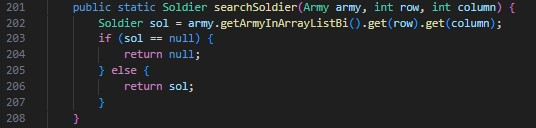
\includegraphics[width=1\textwidth,keepaspectratio]{img/search.jpg}
		%\includesvg{img/automata.svg}
		%\label{img:mot2}
		%\caption{Product backlog.}
	\end{figure}
	
	\begin{figure}[H]
		\centering
		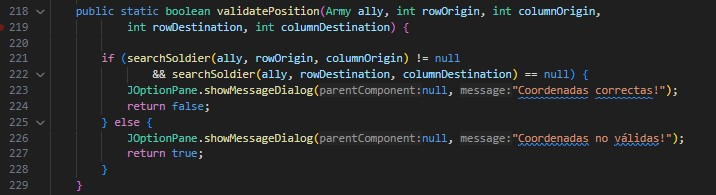
\includegraphics[width=1\textwidth,keepaspectratio]{img/validate.jpg}
		%\includesvg{img/automata.svg}
		%\label{img:mot2}
		%\caption{Product backlog.}
	\end{figure}
	
	
		\begin{figure}[H]
		\centering
		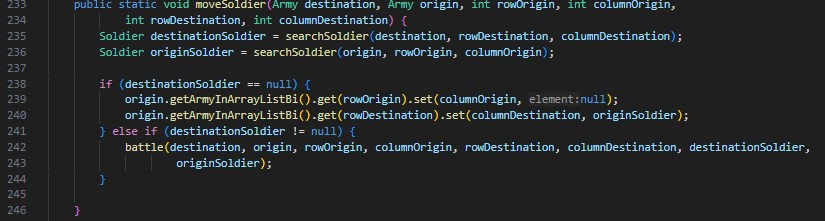
\includegraphics[width=1\textwidth,keepaspectratio]{img/move.jpg}
		%\includesvg{img/automata.svg}
		%\label{img:mot2}
		%\caption{Product backlog.}
	\end{figure}
	
	
	
	\begin{figure}[H]
		\centering
		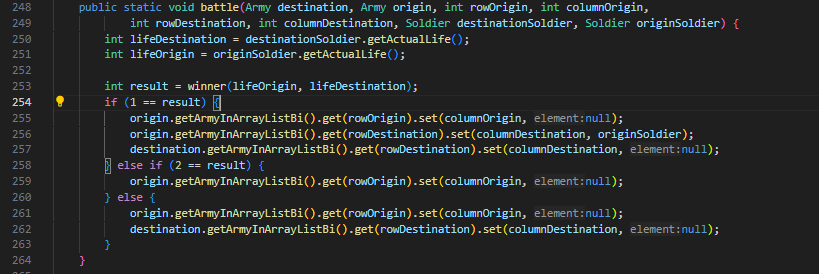
\includegraphics[width=1\textwidth,keepaspectratio]{img/battle.png}
		%\includesvg{img/automata.svg}
		%\label{img:mot2}
		%\caption{Product backlog.}
	\end{figure}
	
	
	
		\begin{figure}[H]
		\centering
		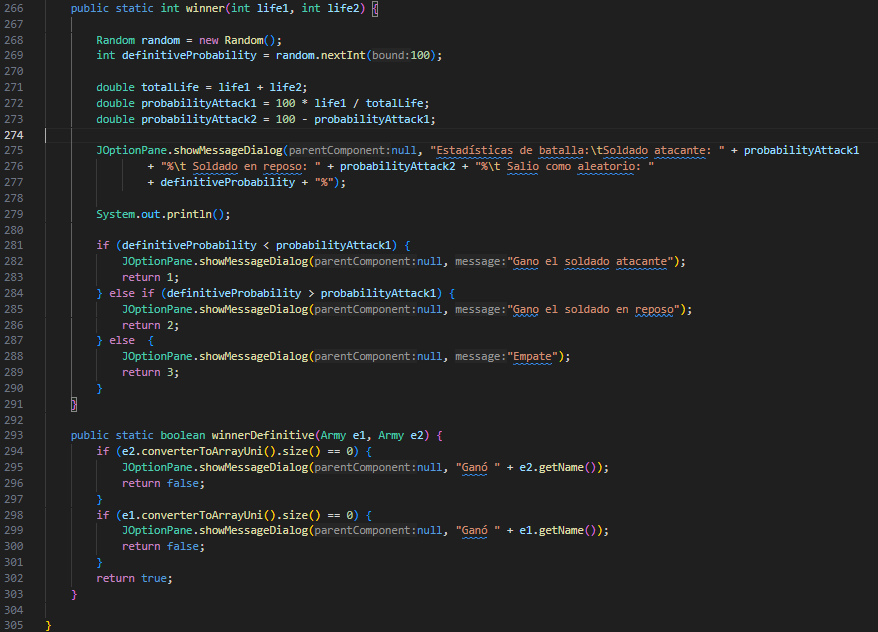
\includegraphics[width=1\textwidth,keepaspectratio]{img/winner.png}
		%\includesvg{img/automata.svg}
		%\label{img:mot2}
		%\caption{Product backlog.}
	\end{figure}
	
	
	
	\subsection{Probando el juego}
	
	
	
	\begin{figure}[H]
		\centering
		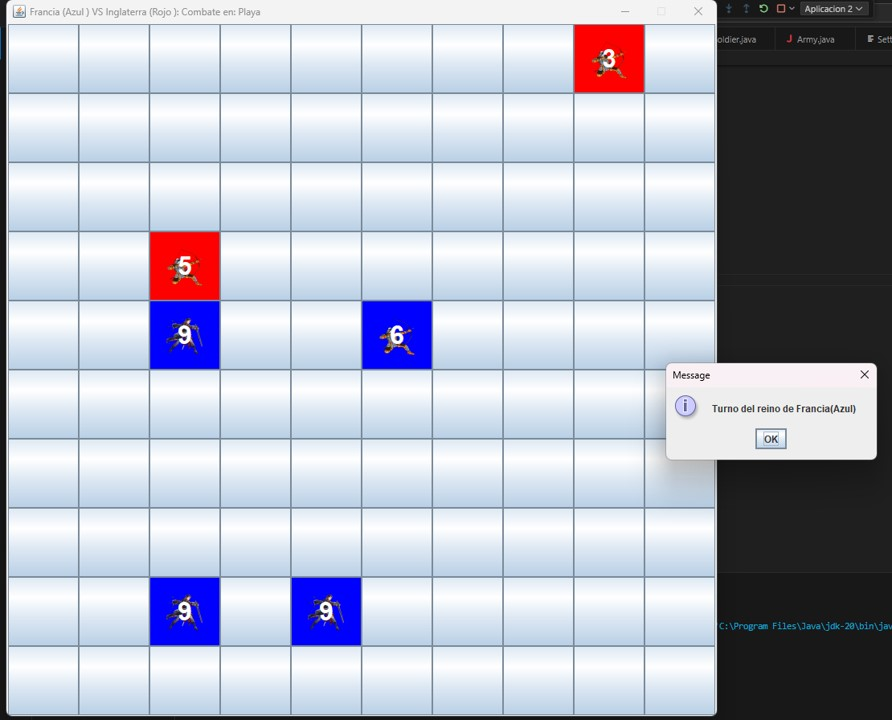
\includegraphics[width=1\textwidth,keepaspectratio]{img/test.jpg}
		%\includesvg{img/automata.svg}
		%\label{img:mot2}
		%\caption{Product backlog.}
	\end{figure}
	
	
	
	\subsection{Diagrama UML}
	
	\begin{figure}[H]
		\centering
		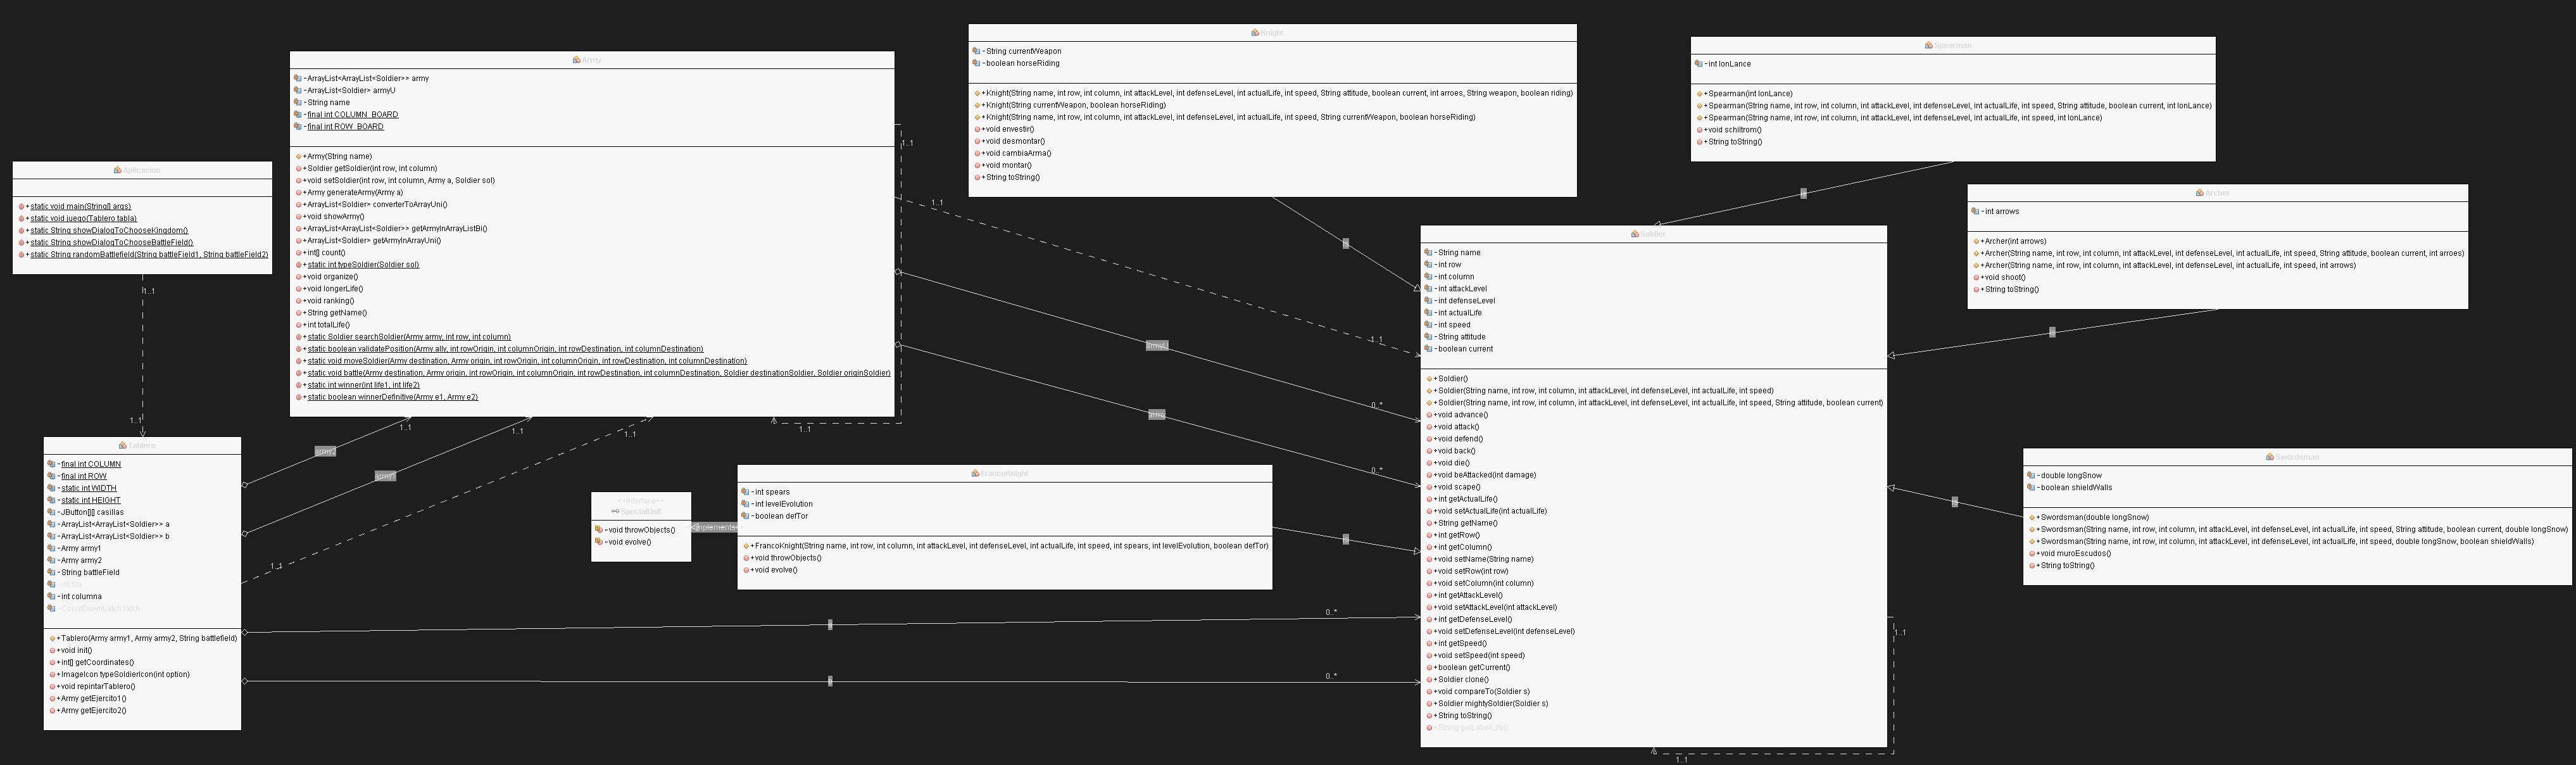
\includegraphics[width=1\textwidth,keepaspectratio]{img/uml.png}
		%\includesvg{img/automata.svg}
		%\label{img:mot2}
		%\caption{Product backlog.}
	\end{figure}
	
	\begin{itemize}	
			\item Si hay problemas en la visualización, puede ver la imagen en la carpeta img (descárgela)
	\end{itemize}
	
	
	
	
	
	\subsection{Estructura de laboratorio 22}
	\begin{itemize}	
		\item El contenido que se entrega en este laboratorio es el siguiente:
	\end{itemize}
	


	\begin{figure}[H]
		\centering
		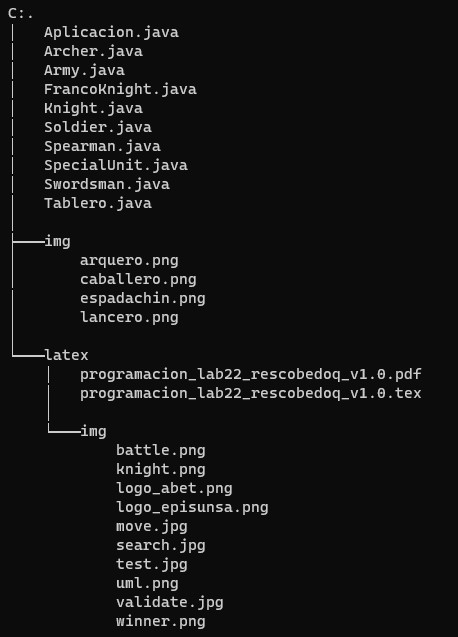
\includegraphics[width=0.8\textwidth,keepaspectratio]{img/tree.jpg}
		%\includesvg{img/automata.svg}
		%\label{img:mot2}
		%\caption{Product backlog.}
	\end{figure}	
	
	\begin{itemize}	
		\item Debido a problemas en la codificación de latex con ciertos caracteres que genera el comando tree f, se opta 
		por enviar la estructura de este laboratorio en formato de imagen
	\end{itemize}
	

   
	
	\section{\textcolor{red}{Rúbricas}}
	
	\subsection{\textcolor{red}{Entregable Informe}}
	\begin{table}[H]
		\caption{Tipo de Informe}
		\setlength{\tabcolsep}{0.5em} % for the horizontal padding
		{\renewcommand{\arraystretch}{1.5}% for the vertical padding
			\begin{tabular}{|p{3cm}|p{12cm}|}
				\hline
				\multicolumn{2}{|c|}{\textbf{\textcolor{red}{Informe}}}  \\
				\hline 
				\textbf{\textcolor{red}{Latex}} & \textcolor{blue}{El informe está en formato PDF desde Latex,  con un formato limpio (buena presentación) y facil de leer.}   \\ 
				\hline 
				
				
			\end{tabular}
		}
	\end{table}
	
	\clearpage
	
	\subsection{\textcolor{red}{Rúbrica para el contenido del Informe y demostración}}
	\begin{itemize}			
		\item El alumno debe marcar o dejar en blanco en celdas de la columna \textbf{Checklist} si cumplio con el ítem correspondiente.
		\item Si un alumno supera la fecha de entrega,  su calificación será sobre la nota mínima aprobada, siempre y cuando cumpla con todos lo items.
		\item El alumno debe autocalificarse en la columna \textbf{Estudiante} de acuerdo a la siguiente tabla:
		
		\begin{table}[ht]
			\caption{Niveles de desempeño}
			\begin{center}
				\begin{tabular}{ccccc}
					\hline
					& \multicolumn{4}{c}{Nivel}\\
					\cline{1-5}
					\textbf{Puntos} & Insatisfactorio 25\%& En Proceso 50\% & Satisfactorio 75\% & Sobresaliente 100\%\\
					\textbf{2.0}&0.5&1.0&1.5&2.0\\
					\textbf{4.0}&1.0&2.0&3.0&4.0\\
					\hline
				\end{tabular}
			\end{center}
		\end{table}	
		
	\end{itemize}
	
	\begin{table}[H]
		\caption{Rúbrica para contenido del Informe y demostración}
		\setlength{\tabcolsep}{0.5em} % for the horizontal padding
		{\renewcommand{\arraystretch}{1.5}% for the vertical padding
			%\begin{center}
			\begin{tabular}{|p{2.7cm}|p{7cm}|x{1.3cm}|p{1.2cm}|p{1.5cm}|p{1.1cm}|}
				\hline
				\multicolumn{2}{|c|}{Contenido y demostración} & Puntos & Checklist & Estudiante & Profesor\\
				\hline
				\textbf{1. GitHub} & Hay enlace URL activo del directorio para el  laboratorio hacia su repositorio GitHub con código fuente terminado y fácil de revisar. &2 &X &2 & \\ 
				\hline
				\textbf{2. Commits} &  Hay capturas de pantalla de los commits más importantes con sus explicaciones detalladas. (El profesor puede preguntar para refrendar calificación). &4 &X &4 & \\ 
				\hline 
				\textbf{3. Código fuente} &  Hay porciones de código fuente importantes con numeración y explicaciones detalladas de sus funciones. &2 &X &2 & \\ 
				\hline 
				\textbf{4. Ejecución} & Se incluyen ejecuciones/pruebas del código fuente  explicadas gradualmente. &2 &X &2 & \\ 
				\hline			
				\textbf{5. Pregunta} & Se responde con completitud a la pregunta formulada en la tarea.  (El profesor puede preguntar para refrendar calificación).  &2 &X &2 & \\ 
				\hline	
				\textbf{6. Fechas} & Las fechas de modificación del código fuente estan dentro de los plazos de fecha de entrega establecidos. &2 &X &2 & \\ 
				\hline 
				\textbf{7. Ortografía} & El documento no muestra errores ortográficos. &2 &X &2 & \\ 
				\hline 
				\textbf{8. Madurez} & El Informe muestra de manera general una evolución de la madurez del código fuente,  explicaciones puntuales pero precisas y un acabado impecable.   (El profesor puede preguntar para refrendar calificación).  &4 &X &2 & \\ 
				\hline
				\multicolumn{2}{|c|}{\textbf{Total}} &20 & &18 & \\ 
				\hline
			\end{tabular}
			%\end{center}
			%\label{tab:multicol}
		}
	\end{table}
	
	\clearpage
	
	\section{Referencias}
	\begin{itemize}			
		\item \url{https://www.geeksforgeeks.org/insertion-sort/}
	\end{itemize}	
	
	%\clearpage
	%\bibliographystyle{apalike}
	%\bibliographystyle{IEEEtranN}
	%\bibliography{bibliography}
	
\end{document}